u\chapter{Rapport technique}

\section{Conception}

\subsection{L'architecture de Qt}

Qt impose un très grand nombre de contraintes par rapport aux classes à utiliser et à leur connexion.
Il n'est pas possible de décider de l'organisation des classes de l'application sans connaître celle de Qt.
L'étape de conception de l'application s'est dû d'être réalisée après l'apprentisage de la librairie.
\paragraph{}

Qt est fortement basé sur le patron MVC \emph{Modèle-vue-contrôleur}, tout l'architecture du programme en dépend.
\paragraph{}

La librairie Qt se décompose en plusieurs parties :
\begin{itemize}
\item \emph{Les modèles}, contenants les données de l'application ;
\item \emph{Les vues}, qui peuvent être générées automatiquements à partir d'un même modèle ;
\item \emph{Un système d'écoute d'évenements} aux travers des signaux/slots propre à Qt.
\end{itemize}

\paragraph{}
Le principe est de générer un unique modèle qui sera affiché par les différenteces la vue.
Les évenements décanchés sur les différentes vues par l'utilsateur sont traités pour modifier le modèle, puis la vue est rafraichie.
La partie \emph{contrôleur} est intégrée aux classes de la vue car le système de slots/signaux que propose Qt est propre et peu encombrant.

\subsection{Modèle de classe}
Toutes les classes héritent de celles de Qt. La librarie impose que toutes les vues doivent hériter du type de vue de Qt voulu (Vue arborescente, editeur de texte, bouton...), qui héritent elles-même de de la classe QWidget.

\paragraph{}
Le programme se compose ainsi des classes principales suivantes :
\begin{itemize}
\item \emph{MainWindow}, contenant des pointeurs vers toutes les vues ainsi que la barre de menu et celle des boutons ;
\item \emph{ModeleXml}, contenant les données de l'arbre XML à jour et toutes les méthodes nécessaire à sa modification ;
\item \emph{Notepad}, la vue des éditeurs de textes (XML et Schéma) ;
\item \emph{Arbo}, la vue de l'arboresence ;
\item \emph{Logger}, la vue du logger ;
\item Et tout un tas des sous classes conçues au fil de la phase de développement dans un soucis de clareté du code.
\end{itemize}

\paragraph{}
L'organisation de l'architecture se résume dans le diagramme de classe qui suit. Seules les composantes principales du programme apparaisent.

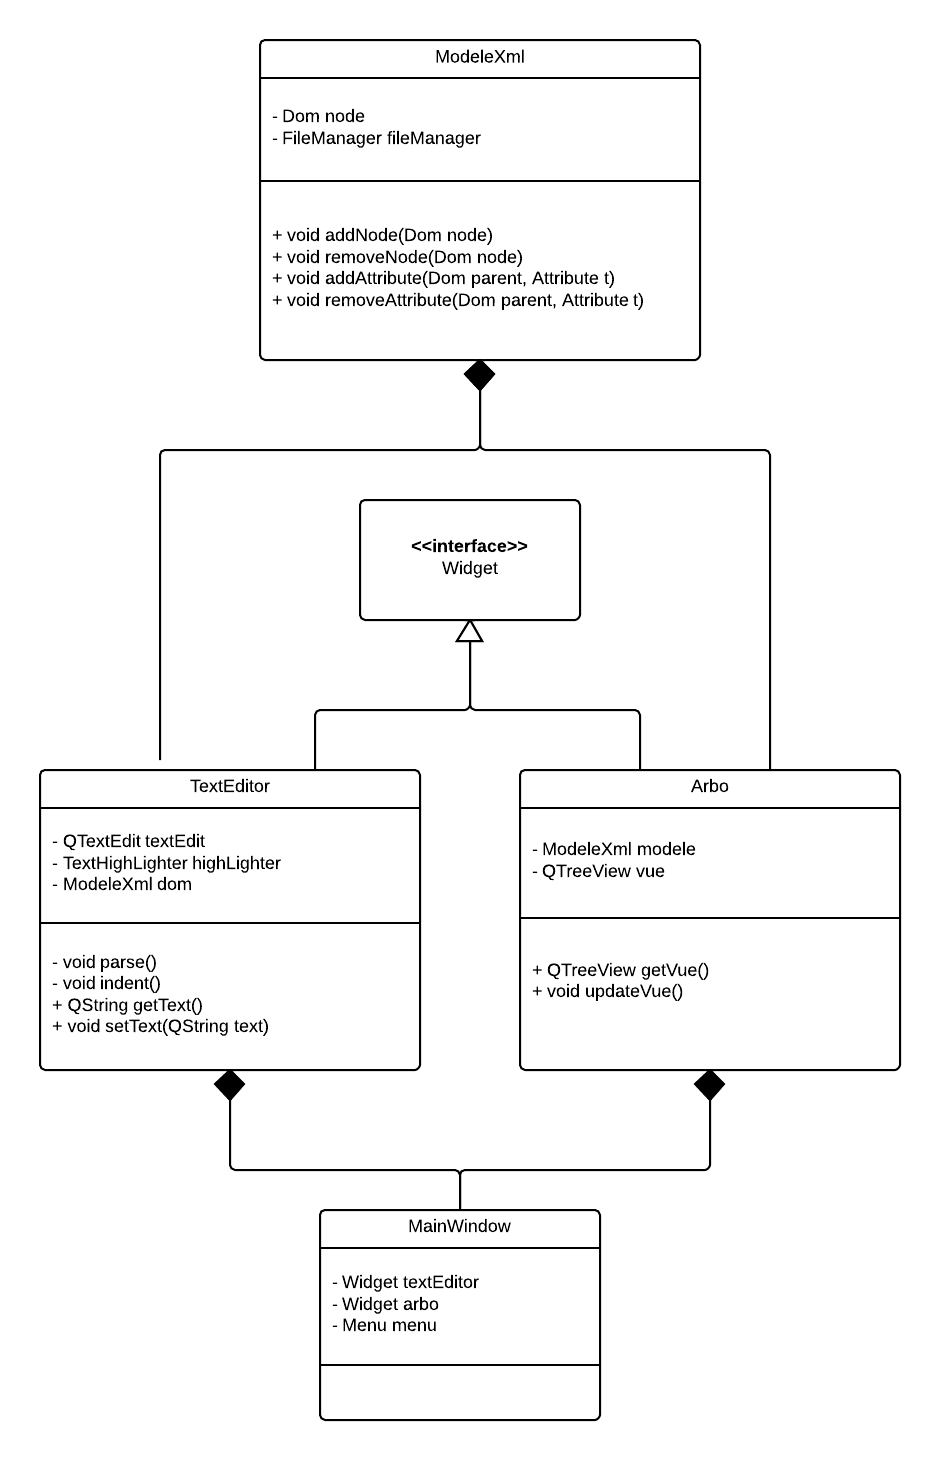
\includegraphics[scale=0.4]{images/classes.png}

\section{Architecture de l'application}
\subsection{Le modèle}

\subsubsection{Structure XML}

Le programme est composé d'un et d'un seul modèle représentant le fichier XML arborescent.
Il contient les informations sur tous les noeud de la structure XML (Nom, valeur, attributs).
L'accès à l'arborscence XML se fait à partir d'un unique attribut noeud parent de type \emph{QDomDocument}, 

\paragraph{}
Au lancement du programme, un dom vide est est généré. Il est redéfinit à l'ouverture d'un fichier de façon automatique grâce à une simple méthode de Qt de la façon suivante.

\begin{lstlisting}
QFile file(currentFile);

if (file.open(QIODevice::ReadOnly))
{
    QString data(file.readAll());

    if (doc->setContent(data, &error, &errorLine, &errorColumn))
    {
        // Definition du dom a partir du texte du fichier
        this->modele->setFromDocument(doc);
    }

    notepad->setText(data);
}
\end{lstlisting}

\subsubsection{Modification}

Le modèle implémente toutes les méthodes nécessaires à la modification du dom. On les retrouve clairement dans le fichier entête de la classe.


\begin{lstlisting}
/**
   @action Modifie le nom du noeud passe en parametre,
   et envoi le signal onNodeNameUpdate
*/
void updateNodeName(QDomNode n, QString newName);

/**
   @action Insere un noeud dans le parent indique,
  et envoi le signal onNodeInsert
*/
void insertNode(QDomNode parent, QDomNode node);

/**
  @action Supprime le noeud et sa sous arborescente
  et envoi le signal onNodeRemove
*/
void removeNode(QDomNode dom);
\end{lstlisting}

Toutes ces méthodes publiques sont appelés par les différentes vues.
Elles modifient directement la structure XML du modèle, puis notifient les changements par un signal.
Cet ensemble est minimal mais suffisant et permet de modifier à souhait l'arbre.
Par exemple une procédure de déplacement d'un noeud pourra être scriptée par une insertion/suppresion.

\subsubsection{Aspect algorithmique}
Toute la subtilité technique de la classe du modèle repose sur la modification propre et optimisée de l'arborescence.
Différents algorithmes de parcours d'arbres ont été utilisés pour y parvenir. Voici par exemple une méthode utilitaire permettant de récupérer la pile représentant le parcours à effectuer en largeur à partir du noeud voulu.

\begin{lstlisting}
stack<int> ModeleXml::pathFromRoot(QDomNode n)
{
    stack<int> s;
    while(!n.parentNode().isNull())
    {
        s.push(rowFromNode(n)); // On recupere la position du noeud en largeur
        n = n.parentNode();
    }

    return s;
}
\end{lstlisting}

\subsection{La vue arborescence}

La classe de la vue arborsecente encapsule la classe QTreeView de Qt permetant de générer une interface arborsence
intéractive avec toutes les options nécessaires (Renommage, suppresion, glisser/déposer...).

\begin{figure}[h!]
\begin{minipage}[b]{\linewidth}
\centering 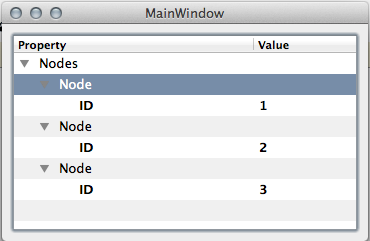
\includegraphics[scale=0.5]{images/arbo.png}
\caption{Vue arborescente de Qt}
\label{arbo}
\end{minipage}
\end{figure}


\subsection{L'éditeur de texte}

L'éditeur de texte est décomposé en deux parties, l'éditeur de schéma et d'éditeur XML. Ce sont en réalité des spécialisation de la classe TextEditor, mais parlons d'abord de l'éditeur de texte en général.
\subsubsection{La classe TextEditor}
C'est ici que sont toutes les méthodes servant à l'édition du texte en général, telle que l'insertion de texte, l'indentation ou la coloration. L'éditeur de texte est une sous classe de QTextEdit, qui fournit toutes les fonctionnalités basiques d'une éditeur de texte riche, telles que la sélection de texte, la copie, l'annulation etc. On peut intégrer plusieurs fonctionnalités à un QTextEdit comme par exemple la coloration syntaxique. Nous parlerons dans un premier temps des fonctionnalités propres à notre éditeur de texte, puis nous verrons plus en détail chacune de ses implémentations, à savoir l'éditeur XML et l'éditeur de schéma.

\paragraph{}
Qt propose un QCompleter, il ne peut cependant pas s'intégrer et proposer l'auto-completion dans un QTextEdit. Même s'il ne s'intègre pas dans un QTextEdit, le QCompleter peut tout de même proposer une suggestion si on lui fourni un début de mot. On peut donc récupérer le mot sous le curseur, le donner au QCompleter et insérer le mot complété dans notre éditeur de texte. Cela se fait de la manière suivante :

\begin{lstlisting}
  //on donne le mot sous le curseur au QCompleter
  completer->setCompletionPrefix(textUnderCursor());
  //on recupere le mot propose
  QString completion = completer->currentCompletion();
  QString currentWord = textUnderCursor();

  //si un mot est sous le curseur et qu'il n'est pas deja complete
  if(currentWord.size() > 0 && currentWord.size() < completion.size())
  {
    QTextCursor cursor = text->textCursor();
    //sauvegarde de la position actuelle du curseur
    int pos = cursor.position();
    //deplacement jusqu'a la fin du mot
    while(word.indexIn(cursor.selectedText()) == 0)
    {
      cursor.movePosition(QTextCursor::Left, QTextCursor::KeepAnchor);
    }
    //insertion de la partie qui n'est pas deja ecrite
    cursor.insertText(completion.right(completion.size() - currentWord.size()));
    //le curseur est replace a sa posision originelle
    cursor.setPosition(pos, QTextCursor::KeepAnchor);
    text->setTextCursor(cursor);
\end{lstlisting}
\paragraph{}
Il n'est pas possible d'intégrer directement l'auto-completion, mais on peut en revanche facilement lier un colorateur syntaxique à un QTextEdit. Qt propose une classe abstraite QSyntaxHighLighter qu'il faut implémenter en y indiquant nos règles de coloration. Le QTextEdit appelle automatiquement la méthode \textit{highlightBlock} du QSyntaxHighLighter dans laquelle on aura indiqué nos règles.

\begin{lstlisting}
  void TextHighLighter::highlightBlock(const QString &text)
  {
    setCurrentBlockState(previousBlockState());
    //l'ordre est important
    //il ne faut pas appliquer de coloration a l'interieur
    //il faut donc colorer les commentaires en premier
    for (int i = 0; i < text.length(); ++i)
    {
      //colore les commentaires
      if(cComment(last, text, i));
      //colore le texte entre quotes
      else if(cQuote(last, text, i));
      //colore les attributs
      else if(cInMarkupAttr(last, text, i));
      //colore les balises
      else if(cMarkup(last, text, i));
    }
  }
\end{lstlisting}
\paragraph{}
Voici par exemple la méthode qui permet de colorer les commentaires :
\begin{lstlisting}
  bool TextHighLighter::cComment(int &last, const QString &text, int i)
  {
    //si on se trouve deja dans un commentaire
    if(currentBlockState() == COMMENT_STATE)
    {
      //si on trouve la fin du commentaire
      if (text.mid(i, 3) == "-->")
      {
        //on colore entre last et la fin du commentaire
        setTextColor(last, i + 4, Qt::gray);
        setCurrentBlockState(DEFAULT_STATE);
      }
      setTextColor(last, i + 1, Qt::gray);
      return true;
    }
    //si on trouve le debut d'un commentaire
    else if (text.mid(i, 4) == "<!--")
    {
      //on sauvegarde la position du debut de commentaire
      last = i;
      //on marque que l'on est dans un commentaire
      setCurrentBlockState(COMMENT_STATE);
      return true;
    }
    return false;
  }
\end{lstlisting}
\paragraph{}
\subsubsection{La classe XmlEditor}

C'est donc une sous classe de TextEditor. Nous avons fait le choix de représenter les données de l'éditeur de texte simplement par une QString, pas de référence vers la position d'un noeud ou d'information supplémentaire comme sa taille ou la délimitation de son contenu.
Un noeud étant identifié par son chemin depuis la racine, il faut reconstruire l'arborescence XML à partir de la QString. Cela se fait à travers la classe QXmlStreamReader qui s'utilise de la manière suivante :
\begin{lstlisting}
  //creation d'un QXmlStreamReader affecte du texte du QTextEdit
  QXmlStreamReader xml(text->toPlainText());
  while(!xml.atEnd())
  {
    //detection d'une balise ouvrante
    if(xml.isStartElement())
    {
      //traitement
    }
    //detection d'une balise fermante
    else if(xml.isEndElement())
    {
      //traitement
    }
  }
\end{lstlisting}
\paragraph{}
On utilise une structure de pile lors de parcours de l'arborescence. On empile l'indice du sommet lorsque l'on rencontre une balise ouvrante et on dépile lorsque l'on rencontre une balise fermante.
On parvient ainsi à se déplacer et à se repérer dans la QString.

Voici le pseudo code de l'algorithme permettant de parcourir l'arbre pour se rendre sur le noeud désiré.

\begin{verbatim}
//noeud que l'on doit trouver dans la QString
var noeudCible
var pile

//Parseur xml de Qt
var xml

Tant que l'on a pas parcouru tout l'arbre
    Si on rencontre une balise ouvrante
        Si la dernière balise rencontrée est une balise ouvrante
            Empiler 0 dans pile
        Sinon
            //c'est que l'on a atteint le fils suivant
            Incrementer le sommet de la pile de 1
        Fin Si
    Sinon Si on rencontre une balise fermante
        Dépiler pile
    Fin Si
    
    Si noeudCible = pile
        Appeler la fonction qui traitera le noeud
        //on arrête le parcours de l'arbre
        retourner
    Fin Si
   
    Sauvegarder la derière balise renconcrée
    Aller à la balise suivante
Fin Tant Que
\end{verbatim}

Cette méthode de parcours de l'arbre est appelée lorsqu'un noeud est inséré, déplacé ou supprimé dans l'arborescence. Elle est utilisée de la manière suivante :

\begin{lstlisting}
  //methode appelee lorsque l'utilisateur renomme un noeud dans l'arborescence
  //on passe en parametre un pointeur de fonction
  xmlEditor->parseDom(n, n.nodeName(), QString(newName), &XmlEditor::updateNodeName);
\end{lstlisting}
\paragraph{}
Voici l'implémentation de l'appel de fonction dans le pseudo code du parcours de document :
\begin{lstlisting}
  
  //si le chemin du node courant est le meme que celui
  //du sommet passe en parametre
  if(cmpVectors(path, nodePath))
  {
    //on appelle la fonction passee en parametre
    //elle traitera le node avec des effets de bord
    if((this->*function)(nbFound, begin, end, c, oldName, newName, xml))
    {
      //on arrete le parcours de l'arbre si la fonction retourne true
      return;
    }
  }
\end{lstlisting}
\paragraph{}
Voici le prototype de la fonction \textit{parseDom} avec la fonction qu'elle prend en paramètre et les fonctions de manipulation de noeud qu'elle peut prendre en paramètre.

\begin{lstlisting}
  //parse le dom jusqu'a trouver le node target
  void parseDom(QDomNode &target, QString oldName, QString newName, bool (XmlEditor::*function)
  (int &nbFound, int &begin, int &end, QTextCursor &c, QString oldname, QString newname, QXmlStreamReader &xml));
  
  //remplace le nom de la balise oldName par newName
  bool updateNodeName(int &nbFound, int &begin, int &end, QTextCursor &c, QString oldName, QString newName, QXmlStreamReader &xml);
  //supprime le noeud
  bool deleteNode(int &nbFound, int &begin, int &end, QTextCursor &c, QString oldName, QString newName, QXmlStreamReader &xml);
  //sauvegarde les donnees du noeud dans le cas d'un deplacement
  bool saveNodeData(int &nbFound, int &begin, int &end, QTextCursor &c, QString oldName, QString newName, QXmlStreamReader &xml);
  //insere un noeud
  bool insertNodeText(int &nbFound, int &begin, int &end, QTextCursor &c, QString oldName, QString newName, QXmlStreamReader &xml);
\end{lstlisting}
\paragraph{}
Ces fonctions manipulent le texte à travers un QTextCursor qui permet de naviguer dans un QTextEdit. Un QTextCursor permet notamment de se déplacer de mot en mot, d'aller à la fin de la ligne ou d'aller à la ligne suivante. Un outil donc indispensable dans la manipulation du texte.

\paragraph{}
La liaison vers un schéma se fait à l'aide d'expressions régulières. Le XML étant standardisé, les données auront toujours la même forme, une expression régulière semble donc le plus simple pour trouver une information dans du texte.

\begin{lstlisting}
  void XmlEditor::removeSchema()
  {
    QString s(text->toPlainText());
    //regex du lien vers un schema
    QRegExp r("\n*xmlns:xsi.*=\".*\.xsd\"\n*");
    suppression de la regex dans le texte
    s.remove(r);
    text->setText(s);
  }
\end{lstlisting}
\paragraph{}
Il est intéressant de noter que l'on utilise une fois de plus la classe QXmlStreamReader pour se déplacer dans l'arborescence XML. Le lien vers le schéma se trouve dans la balise racine, le plus simple pour la trouver est donc de parcourir le document jusqu'à la trouver.
\begin{lstlisting}
  while(!xml.atEnd())
  {
    //lorsque l'on trouve la premiere balise ouvrante
    if(xml.isStartElement())
    {
      //on deplace le curseur jusqu'a la position de la fin de cette balise
      moveCursorToLineAndColumn(c, xml.lineNumber() - 1, xml.columnNumber() - 1, false);
      //construction du lien vers le schema
      QString link("\nxmlns:xsi=\"http://www.w3.org/2001/XMLSchema-instance\"\nxsi:noNamespaceSchemaLocation=\"");
      link.append(XmlFileManager::getFileManager()->getSchemaName()).append("\"");
      //insertion du lien dans le document
      c.insertText(link);
      text->setTextCursor(c);
      return;
    }
    xml.readNext();
  }
\end{lstlisting}
\paragraph{}
En plus de créer et supprimer un lien vers un schéma, il est également possible de l'extraire, pour la validation par exemple. Cela se fait une fois de plus grâce à une expression régulière. Il est intéressant de noter dans l'exemple suivant que nous ne gérons que les liens locaux vers un schéma et pas les lien vers un schéma distant.
\begin{lstlisting}
  QString s(text->toPlainText());
  //split du document pour se placer directement a l'endroit du lien
  QStringList l(s.split("xsi:noNamespaceSchemaLocation=\""));
  //si un lien est present dans le document
  if(l.size() > 1)
  {
    //split selon le caractere " pour ne garder que le lien
    s = l.at(1).split("\"").at(0);
    //on retourne le chemin courant du fichier XML auquel on concatene le lien que l'on vient de trouver
    return XmlFileManager::getFileManager()->getCurrentFilePath().append("/").append(s);
  }
  //on cherche s'il n'y a pas de lien distant
  l = s.split("xsi:SchemaLocation=\"");
  if(l.size() > 1)
  {
    //on notifie qu'on ne le gere pas encore s'il existe
    emit log("Cannot process http requests yet, XML will not be checked", QColor("orange"));
  }
  return "";
\end{lstlisting}
\paragraph{}
\subsubsection{La classe SchemaEditor}
La classe SchemaEditor ne rajoute pas vraiment de fonctionnalités à la classe TextEditor mise à part la génération de schéma à partir d'un document XML. Elle fonctionne de manière très simple, les balises sont extraites du document XML et sont ajoutées au schéma. L'extraction des balises se fait à nouveau grâce à la classe QXmlStreamReader, on parcourt le document et ajoute chaque balise dans une liste si elle n'est pas déjà présente

\begin{lstlisting}
  while(!xml.atEnd())
  {
    //on utilise une hashmap pour simplifier la non duplication
    h.insert(xml.name().toString(), 0);
    xml.readNext();
  }
  //on appelle la methode de generation de schema
  schemaEditor->genSchema(h.keys());
\end{lstlisting}
\paragraph{}
Voici l'implémentation de la méthode de génération de schéma, on peut remarquer qu'elle est assez basique et laisse à l'utilisateur le soin de compléter la valeur et le type de chaque élément.
\begin{lstlisting}
  void DtdEditor::genSchema(QList<QString> l)
  {
    //ajout des meta data
    text->setText("<?xml version=\"1.0\" encoding=\"UTF-8\" ?>");
    text->append("<xs:schema xmlns:xs=\"http://www.w3.org/2001/XMLSchema\">");

    //ajout de chaque element
    for(QString s : l)
    {
      QString toAppend("<xs:element name=\"");
      toAppend.append(s).append("\"/>");
      text->append(toAppend);
    }
    text->append("</xs:schema>");
    indent();
  }

\end{lstlisting}
\paragraph{}
\subsubsection{La validation}
Parlons maintenant de la validation syntaxique et sémantique. La validation syntaxique se fait très simplement à l'aide du QXmlStreamReader, qui permet de détecter une erreur et d'indiquer la ligne, ainsi que le type de l'erreur.

\begin{lstlisting}
  while(!xml.atEnd())
  {
    xml.readNext();
    //si le parseur XML rencontre une erreur
    if(xml.hasError())
    {
      //affichage de la ligne de l'erreur avec son type
      emit log("Erreur ligne " + QString::number(xml.lineNumber()) + " : " + xml.errorString(), QColor("red"));
    }
  }
\end{lstlisting}
\paragraph{}
Pour la validation sémantique, qui ne peut se faire que si un schéma est rattaché au document XML, on doit passer par une autre classe de Qt, le QXmlSchemaValidator et sa méthode validate. Nous l'utilisons le la manière suivante :
\begin{lstlisting}
  QXmlSchema schema;
  //extraction de l'url du schema dans le document XML
  QString url(extractSchemaUrl());

  //si le xml contient une url valide vers un schema
  if(url.size() > 1)
  {
    schema.load(QString("file://").append(url));
    //on verifie au passage la validite du schema en lui meme
    if (schema.isValid())
    {
      emit log("Schema XSD valide", QColor("green"));
      QXmlSchemaValidator validator(schema);
      validator.setMessageHandler(mh);
      if (validator.validate(this->getText().toUtf8(), QUrl(XmlFileManager::getFileManager()->getCurrentSchema())))
      {
        //notification que la semantique est valide
        emit log("Semantique XML valide", QColor("green"));
      }
    }
    return true;
  }
  //si le schema n'a pas pu etre trouve
  emit log("Schema XSD invalide, est-il manquant ou invalide ?", QColor("orange"));
\end{lstlisting}
\paragraph{}
\subsection{Le logger}
Le logger est la partie que reçoit tous les messages pour les afficher à l'utilisateur. Il repose fortement sur le principe de signaux et de slots de Qt. Le fonctionnement est les suivant : Qt propose de connecter un objet émetteur, qui enverra des messages avec la macro \textit{emit} sur le slot d'un objet receveur, qui est en réalité une fonction qui sera appelée au moment du \textit{emit}. Voici par exemple le fonctionnement de l'envoi de messages à afficher :

\paragraph{}
Tout d'abord l'interface de notre Logger, pour montrer que les slots ne sont rien d'autres que des fonctions.
\begin{lstlisting}
  class Logger : public QWidget
  {
    Q_OBJECT
    public:
    explicit Logger();
    
    signals:
    //les signaux, il n'y en a aucun dans notre Logger
    
    public slots:
    //notre slot log qui affichera dans la zone de texte la QString de la couleur QColor
    void log(QString s, QColor c);

    private slots:
    //slots prives, on ne pourra connecter que des signaux de la classe sur des slots de cette meme classe

    private:
    //attributs prives
  };
\end{lstlisting}
\paragraph{}
On connecte les objets entre eux grâce à la fonction \textit{connect(sender, signal, receiver, slot)} de Qt.
\begin{lstlisting}
  //on connecte l'editeur de texte avec le logger sur le slot log
  connect(notepad, SIGNAL(log(QString,QColor)), logger, SLOT(log(QString,QColor)));
\end{lstlisting}
\paragraph{}
Et lorsque qu'il y aura un \textit{emit} du signal \textit{log}, la fonction correspondante, dans notre cas \textit{log} sera appelée.

\begin{lstlisting}
  //l'emission du signal dans la methode de validation semantique
  emit log("Semantique XML valide", QColor("green"));
  //appelera automatiquement
  void Logger::log(QString s, QColor c)
  {
    //changement de la couleur d'affichage en la couleur desiree
    logArea->setTextColor(c);
    QTextCursor cursor = logArea->textCursor();
    //insertion du texte dans le QTextEdit qui sert de zone d'affichage au logger
    cursor.insertText(s);

    logArea->setTextCursor(cursor);
    //affichage du Logger s'il etait masque
    show();
  }
\end{lstlisting}
\paragraph{}
Ce système de signal/slot est énormément utilisé pour faire communiquer nos widgets les uns avec les autres, et permet d'une part de les séparer, c'est à dire que l'arborescence ne possède pas de pointeur vers l'éditeur de texte et inversement, mais également de ne pas avoir non plus de pointeur vers le contrôleur, une fois que les connexions sont faites dans le contrôleur, nos widgets peuvent communiquer de manière totalement indépendante.

\subsection{Le gestionnaire de fichiers}
Nous avons fait le choix d'avoir une seule instance du gestionnaire de fichier, et de s'en servir pour stocker le modèle et les différents documents ouverts. Le gestionnaire de fichier est donc un singleton. 
\paragraph{}
Il embarque les fonctionnalités basiques d'un gestionnaire de fichier, telles que l'ouverture et la sauvegarde. C'est à travers ce gestionnaire de fichiers que l'on va gérer les deux documents ouverts, le document XML et le schéma qui lui est associé.

\section{Résultat}
